\chapter{预条件、自适应优化与矩阵更新}
\label{l4:chapter}

\begin{coursebox}{学习目标与课时安排}
本讲安排为一个半理论学时和一个半实验学时。核心问题是：参数空间中什么叫“一小步”，不同的定义如何产生不同更新方向？理论核心依次是二次度量、对偶范数、谱范数球与 polar 方向；AdaGrad、AdamW 和 Muon 用于说明这些理想模型如何进入带有历史状态的实际算法。

自然梯度、K-FAC、Shampoo 以及更新相关性的稳态推导列为选读。实验必须区分精确 SVD 参考、有限步 Newton--Schulz 近似、辅助参数更新和学习率尺度约定。学完本讲，应能从一个更新公式识别其几何、历史状态和数值近似，并能设计公平的优化器比较。
\end{coursebox}

\section{同一个梯度，什么叫同样大小的一步}
\label{l4:metric}

设目标为 $F(w)$，当前梯度为 $g=\nabla F(w)$。一阶近似告诉我们，小位移 $d$ 引起的损失变化约为 $\inner{g}{d}$，但只最小化这个线性函数会沿某个方向无限前进。下降方法必须限制位移，或者惩罚过大的位移。限制的方式决定了“最陡”的含义。

先考虑二次惩罚模型
\begin{equation}
 d_\star=\argmin_{d\in\R^p}
 \left\{\inner{g}{d}+\frac1{2\eta}d^\top M d\right\},
 \qquad M\succ0.
 \label{l4:quadratic-model}
\end{equation}
对 $d$ 求导可得唯一解
\begin{equation}
 \boxed{d_\star=-\eta M^{-1}g=-\eta Pg},\qquad P=M^{-1}.
 \label{l4:preconditioned-step}
\end{equation}
矩阵 $M$ 定义了位移的度量，$P$ 是预条件矩阵。$M=I$ 给出普通梯度下降；$M$ 在某一方向大，表示该方向的位移昂贵，因此相应更新更小。这里 $M$ 必须正定，否则二次模型不一定有有限最小值。

若使用变量替换 $z=M^{1/2}w$，在 $z$ 坐标中进行普通梯度下降，再换回 $w$，恰好得到式\eqref{l4:preconditioned-step}。因此预条件也可理解为选择适合问题的坐标。它不会改变目标函数的最优解集合，却会改变达到最优解的路径与速度；在欠定或非凸问题中，路径变化还可能影响最终选中的解。

\subsection{曲率与稳定性如何变化}

对固定二次目标 $F(w)=\tfrac12(w-w_\star)^\top H(w-w_\star)$，设 $H\succ0$ 且 $P\succ0$ 固定。误差更新为
\[
 e_{t+1}=(I-\eta PH)e_t.
\]
虽然 $PH$ 不必对称，它与对称正定矩阵 $P^{1/2}HP^{1/2}$ 相似。因此迭代的稳定条件为
\begin{equation}
 0<\eta<\frac{2}{\lambda_{\max}(P^{1/2}HP^{1/2})}.
 \label{l4:preconditioned-stability}
\end{equation}
有效条件数也由这个矩阵决定。若 $P=H^{-1}$，则全部特征值等于一，$\eta=1$ 一步到达二次目标的最优点。这是 Newton 方法最清楚的理想情形。对非凸目标，Hessian 可能不定；对自适应方法，$P$ 随历史变化，不能直接用一个固定矩阵的结论覆盖整个训练过程\citep{Nocedal2006}。

\begin{example}[改变度量解决各向异性]
令
\[
 F(w)=\frac12(100w_1^2+w_2^2),\qquad w_0=(1,1)^\top.
\]
普通 GD 的稳定步长必须小于 $0.02$。取 $\eta=0.01$，得到
$w_1=(0,0.99)^\top$：陡方向已经到零，平缓方向只前进了百分之一。若使用 $M=\diag(100,1)$ 和 $\eta=1$，则
$d=-M^{-1}\nabla F(w_0)=(-1,-1)^\top$，一步达到零。

这个例子说明预条件的目标是改善相关的曲率比例，而不是单纯让所有坐标更新幅度相同。后面 Adam 的梯度二阶矩与 Hessian 不是同一个量，因此不能把 Adam 的对角分母直接称为 Hessian 的对角近似。
\end{example}

\section{对偶范数与最陡下降方向}
\label{l4:dual-norm}

二次模型是一条路线，另一条路线是给位移一个硬约束。给定一个范数 $\psi$，考虑
\begin{equation}
 \min_{\psi(d)\leq\rho}\inner{g}{d},\qquad\rho>0.
 \label{l4:norm-ball}
\end{equation}
这里使用闭球，使有限维连续优化问题取得最小值。若改成严格不等式 $\psi(d)<\rho$，非零线性目标通常只有下确界而没有最小点。

\begin{definition}[对偶范数]
范数 $\psi$ 的对偶范数为
\begin{equation}
 \psi_*(g)=\max_{\psi(u)\leq1}\inner{g}{u}.
 \label{l4:dual-norm-definition}
\end{equation}
它衡量单位位移预算下，线性目标能够变化多大。
\end{definition}

\begin{proposition}[范数球内的线性最小化]
式\eqref{l4:norm-ball}的最优值是 $-\rho\psi_*(g)$。若
$u_\star\in\argmax_{\psi(u)\leq1}\inner{g}{u}$，则
$d_\star=-\rho u_\star$ 是一个最优解。解不必唯一。
\end{proposition}
\begin{proof}
范数的对称性和变量代换 $d=-\rho u$ 给出
\[
 \min_{\psi(d)\leq\rho}\inner{g}{d}
 =-\rho\max_{\psi(u)\leq1}\inner{g}{u}
 =-\rho\psi_*(g).
\]
有限维闭单位球紧致，连续目标取得最大值，故上述方向存在。
\end{proof}

对 $g\ne0$，几个典型选择为
\begin{center}
\small
\begin{tabularx}{\textwidth}{lXXX}
\toprule
位移约束 & 对偶范数 & 一个最优方向 $d_\star$ & 解释\\
\midrule
$\norm{d}_2\leq\rho$ & $\norm{g}_2$ & $-\rho g/\norm{g}_2$ & 固定总欧氏长度\\
$\norm{d}_\infty\leq\rho$ & $\norm{g}_1$ & $-\rho\operatorname{sign}(g)$ & 各坐标各有预算\\
$\norm{d}_1\leq\rho$ & $\norm{g}_\infty$ & $-\rho\operatorname{sign}(g_j)e_j$ & 预算集中在最大梯度坐标\\
\bottomrule
\end{tabularx}
\end{center}
第三行取 $j\in\argmax_i|g_i|$；并列最大时可以有多个解。第二行在零梯度坐标上也不唯一，约定 $\operatorname{sign}(0)=0$ 即可得到一个解。若 $g=0$，整个约束球都是最优解，不能使用包含 $1/\norm{g}$ 的公式。

\begin{example}[同一个梯度对应三种预算]
令 $g=(3,-1)^\top$，$\rho=0.1$。欧氏球给出
\[
 d_2=\frac{0.1}{\sqrt{10}}(-3,1)^\top,
 \qquad \inner{g}{d_2}=-0.1\sqrt{10}.
\]
无穷范数球给出 $d_\infty=(-0.1,0.1)^\top$，线性变化为 $-0.4$；一范数球给出 $d_1=(-0.1,0)^\top$，线性变化为 $-0.3$。

这不能直接证明其中某个算法更好，因为三种可行集不同。例如 $\norm{d_\infty}_2=\sqrt2\rho$，已经超过欧氏球的半径。比较更新时，应说明保持的是哪一种尺度，不能只比较公式中的同一个 $\rho$ 数值。
\end{example}

\begin{figure}[htbp]
 \centering
 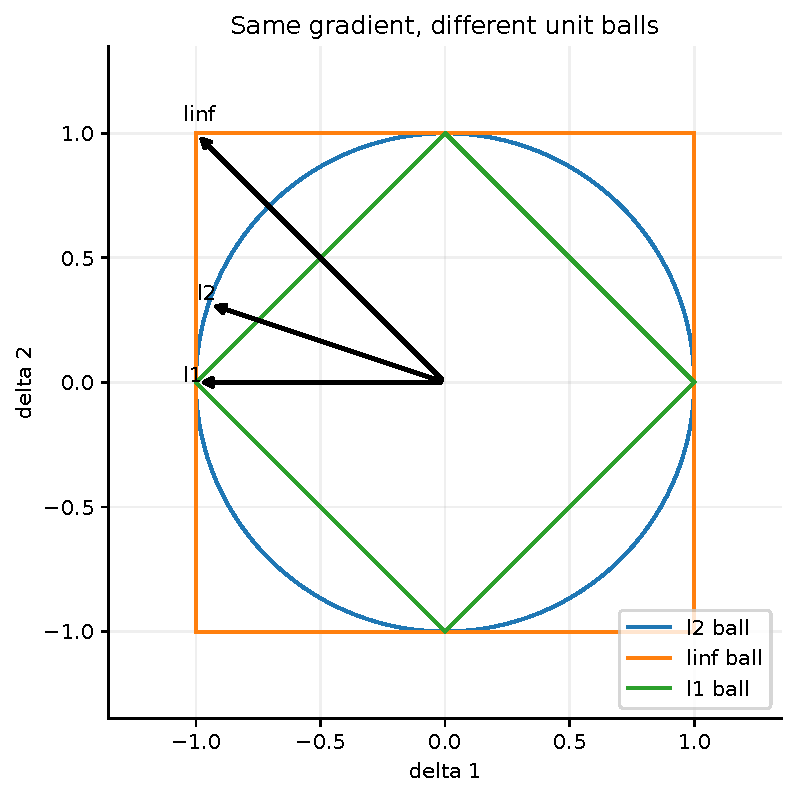
\includegraphics[width=0.7\textwidth]{figures/norm_geometry.pdf}
 \caption{同一梯度在不同闭范数球上的精确线性最小化方向。相同的半径数值对应不同的可行位移集合，因此方向与一阶下降量也不同。这幅图比较的是局部几何模型，完整算法还需指定梯度估计、历史状态和步长。}
 \label{l4:fig-norm-geometry}
\end{figure}

\subsection{方向归一化与普通 GD 的区别}

欧氏球给出的是\emph{归一化梯度方向}，普通 GD 则来自二次惩罚。二者的步长一个控制长度，一个乘在原始梯度上。为了看清一般关系，考虑
\begin{equation}
 \min_d\left\{\inner{g}{d}+\frac{\psi(d)^2}{2\eta}\right\}.
 \label{l4:squared-norm-model}
\end{equation}
对固定半径 $r=\psi(d)$，线性项的最优值为 $-r\psi_*(g)$；再对 $r\geq0$ 最小化
$-r\psi_*(g)+r^2/(2\eta)$，得到
\[
 r_\star=\eta\psi_*(g),\qquad
 d_\star=-\eta\psi_*(g)u_\star.
\]
因此同一个范数，配合固定半径或平方范数惩罚，也会给出不同的更新长度。这是后面统一理解算法时必须保留的细节。

\begin{coursebox}{“范数统一优化器”应当怎样理解}
不同范数定义了几类理想最陡下降方向。实际算法还要指定梯度估计、动量、历史统计量、步长、权重衰减和数值实现。对偶范数可以解释一个方向为什么出现，但仅凭方向相似，不能把两个完整算法的稳定性和收敛定理互相移植。
\end{coursebox}

\section{从累积二阶矩到 Adam}
\label{l4:adaptive}

\subsection{AdaGrad 与 RMSProp 的历史统计量}

为避免时间下标歧义，本节在参数 $w_{t-1}$ 处计算梯度 $g_t$，随后产生 $w_t$，初始状态下标为零。逐元素运算用 $\odot$ 或分量公式表示。
AdaGrad 维护累积平方梯度\citep{Duchi2011}
\begin{equation}
 s_t=s_{t-1}+g_t\odot g_t,
 \qquad
 w_t=w_{t-1}-\eta\frac{g_t}{\sqrt{s_t}+\epsilon},
 \label{l4:adagrad}
\end{equation}
其中分式与平方根都按分量计算，$\epsilon>0$ 用于避免数值除零。长期出现较大梯度的坐标获得较小的有效步长；很少出现梯度的坐标则不会仅因其他坐标更新频繁而被同等压低。其累积结构也会使分母持续增大，是否符合任务需要取决于训练阶段。

RMSProp 用指数平均代替无限累积：
\begin{equation}
 v_t=\beta_2v_{t-1}+(1-\beta_2)g_t\odot g_t,
 \qquad
 w_t=w_{t-1}-\eta\frac{g_t}{\sqrt{v_t}+\epsilon}.
 \label{l4:rmsprop}
\end{equation}
指数平均可以追踪变化的梯度尺度，但有限记忆也改变了理论条件。AdaGrad 的某个收敛证明不能仅将累积和替换成指数平均后原样保留。这里的 $v_t$ 是\emph{梯度平方的统计量}，不是 Hessian 的特征值或方差本身；非零均值时二阶矩与方差也不同。

\subsection{Adam 的完整状态方程}

Adam 同时使用一阶矩和二阶矩状态\citep{Kingma2015}：
\begin{align}
 m_t&=\beta_1m_{t-1}+(1-\beta_1)g_t,\notag\\
 v_t&=\beta_2v_{t-1}+(1-\beta_2)g_t\odot g_t,\notag\\
 \widehat m_t&=\frac{m_t}{1-\beta_1^t},\qquad
 \widehat v_t=\frac{v_t}{1-\beta_2^t},\notag\\
 u_t&=\frac{\widehat m_t}{\sqrt{\widehat v_t}+\epsilon},\qquad
 w_t=w_{t-1}-\eta_tu_t.
 \label{l4:adam}
\end{align}
这里 $m_0=v_0=0$，$0\leq\beta_1,\beta_2<1$。偏差修正补偿零初始状态对恒定均值矩估计的初期影响；它不保证当梯度分布变化时，矩估计就是当前真实矩。

若把 $D_t=\diag(\sqrt{\widehat v_t}+\epsilon)$，则 Adam 更新是
$-\eta_tD_t^{-1}\widehat m_t$。这可以看作对\emph{带记忆的方向}施加对角预条件，不能一般写成对当前真实梯度使用某个 Hessian 逆矩阵。

\subsection{哪些情况下才出现 SignGD}

设 $\beta_1=\beta_2=0$ 且忽略 $\epsilon$，对于非零梯度分量，式\eqref{l4:adam}严格给出
\[
 u_t=\frac{g_t}{|g_t|}=\operatorname{sign}(g_t).
\]
零分量约定更新为零。另一个可检验的特例是从第一步开始梯度始终等于同一个非零常向量，此时偏差修正后 $\widehat m_t=g$、$\widehat v_t=g^2$，也得到 sign 方向。实际训练中可以用这个极限解释逐坐标归一化的倾向，但“目标是二次函数”并不足以使历史梯度保持不变。

\begin{example}[Adam 的方向可以与当前 sign 不同]
考察一个坐标，设 $m_0=v_0=0$、$\beta_1=\beta_2=0.9$，忽略 $\epsilon$。两次梯度分别为 $g_1=1$、$g_2=-0.1$。第二步有
\[
 m_2=0.08,\qquad v_2=0.091,
 \qquad\widehat m_2=\frac{0.08}{0.19},
 \qquad\widehat v_2=\frac{0.091}{0.19}.
\]
因此 $u_2\approx0.6084>0$，Adam 使参数减小；当前梯度为负，SignGD 则使参数增大。两步就足以看出历史状态的重要性。这也不意味着 Adam 在整个过程中一定更差：动量可能暂时抵抗一个新方向；是否有益需要考察后续动力学。
\end{example}

在对角正定二次函数上，固定步长 SignGD 的每个坐标最终进入一个宽度与步长成比例的区间，并通常形成二周期。这是有界性分析，不是收敛到最优点的证明，也不是完整 Adam 的稳定性定理。Adam 的收敛需要额外条件；已有工作给出了简单凸随机优化环境中不能收敛到最优解的反例及相应修正\citep{Reddi2018}。课堂上应以这些反例提醒学生核对假设，不能反过来解释为任何使用 Adam 的训练都会失败。

\subsection{坐标与学习率的单位}

把损失整体乘以正数 $c$，普通 GD 的梯度和位移都会乘以 $c$；在 $\epsilon$ 可忽略且状态同样缩放的理想条件下，Adam 的 $m$ 乘以 $c$、$v$ 乘以 $c^2$，比值近似不变。因此 Adam 与 SGD 的学习率数值不能直接比较。学习率 $10^{-3}$ 比 $10^{-2}$ 小，并不意味着参数实际走得更短。

逐坐标方法也依赖坐标系。例如取 $g=(1,2)^\top$ 和
\[
 Q=\frac1{\sqrt2}
 \begin{pmatrix}1&-1\\1&1\end{pmatrix}.
\]
则 $Q\operatorname{sign}(g)=(0,\sqrt2)^\top$，但
$\operatorname{sign}(Qg)=(-1,1)^\top$。先旋转梯度再取 sign，与先取 sign 再旋转不相同。这不是一个实现缺陷，而是选择坐标范数的几何后果。

\section{AdamW 与自适应 L2 正则}
\label{l4:adamw}

对普通梯度下降，把目标改成 $F(w)+\lambda\norm{w}^2/2$ 会得到
\[
 w_t=(1-\eta_t\lambda)w_{t-1}-\eta_t\nabla F(w_{t-1}).
\]
因此在这一个特定算法中，L2 正则与乘性权重衰减等价。预条件出现后，情况改变。若暂时固定 $P$，耦合 L2 更新是
\begin{equation}
 w_t=w_{t-1}-\eta_tP\bigl(g_t+\lambda w_{t-1}\bigr),
 \label{l4:coupled-l2}
\end{equation}
而解耦衰减是
\begin{equation}
 w_t=(1-\eta_t\lambda)w_{t-1}-\eta_tPg_t.
 \label{l4:decoupled-decay}
\end{equation}
除非预条件与正则形式满足特别关系，两式不同。在 Adam 中，若将 $\lambda w$ 加进梯度，它还会进入 $m_t,v_t$ 的历史统计量，差异更大。

AdamW 用来自原目标梯度的 $u_t$，并另外施加衰减\citep{Loshchilov2019}：
\begin{equation}
 \boxed{w_t=(1-\eta_t\lambda)w_{t-1}-\eta_tu_t}.
 \label{l4:adamw-rule}
\end{equation}
这里约定 $\lambda$ 是与学习率相乘的衰减系数。有些实现直接传入每步收缩量，或对不同参数组设置不同的衰减；比较配置前必须核对定义。

\begin{example}[两种正则化的收缩不同]
取当前 $w=(1,1)^\top$、数据梯度 $g=0$、固定
$P=\diag(0.01,1)$、$\eta=0.1$、$\lambda=1$。
耦合 L2 更新得到 $(0.999,0.9)^\top$，解耦衰减得到 $(0.9,0.9)^\top$。第一种规则在预条件较小的方向上也更少收缩，第二种规则使用相同的相对收缩比例。

这个例子只比较两个明确更新公式，不说明哪一种必然泛化更好。对真实网络，还需说明 bias、归一化参数和输出层是否衰减，以及学习率随时间变化后累计收缩量如何变化。
\end{example}

\section{矩阵参数：谱范数球与 polar 方向}
\label{l4:spectral-ball}

神经网络的一层常由矩阵 $W\in\R^{m\times n}$ 表示。将它展平成向量当然可以使用前面的算法，但矩阵本身还具有输入、输出和奇异方向的结构。记矩阵梯度为 $G$，Frobenius 内积为
$\inner{G}{D}_F=\tr(G^\top D)$。

矩阵谱范数与核范数分别为
\[
 \norm{D}_{\rm op}=\max_{\norm{x}_2\leq1}\norm{Dx}_2,
 \qquad
 \norm{G}_*=\sum_{i=1}^{\rank(G)}\sigma_i(G).
\]
谱范数控制一个线性映射对任何输入方向的最大放大，核范数是其对偶范数。这一对偶关系使矩阵更新具有一个简洁的精确解。

\begin{theorem}[谱范数球内的最优线性方向]
令 $G=U_r\Sigma_rV_r^\top$ 为秩 $r>0$ 的紧致 SVD，$\Sigma_r$ 的对角元严格为正。则
\begin{equation}
 \min_{\norm{D}_{\rm op}\leq\rho}\inner{G}{D}_F
 =-\rho\norm{G}_*,
 \qquad
 D_\star=-\rho U_rV_r^\top
 \label{l4:polar-optimum}
\end{equation}
给出一个最优解。称 $Q(G)=U_rV_r^\top$ 为本讲采用的 canonical polar 方向，并约定 $Q(0)=0$。
\end{theorem}
\begin{proof}
将 $G$ 写成 $\sum_{i=1}^r\sigma_i u_i v_i^\top$，则任意可行 $D$ 满足
\[
 \inner{G}{D}_F=\sum_{i=1}^r\sigma_i u_i^\top Dv_i
 \geq-\sum_{i=1}^r\sigma_i\norm{D}_{\rm op}
 \geq-\rho\sum_{i=1}^r\sigma_i.
\]
对 $D_\star=-\rho U_rV_r^\top$，每个 $u_i^\top D_\star v_i=-\rho$，且其谱范数为 $\rho$，所以达到下界。
\end{proof}

谱范数单位球包含所有收缩映射，\emph{不是正交矩阵集合}。上面的一个最优解恰好把非零梯度奇异方向上的奇异值变为一。若矩阵满秩且 $m\geq n$，有 $Q^\top Q=I_n$；若满秩且 $m\leq n$，有 $QQ^\top=I_m$。秩亏时，这两个乘积对应子空间投影，不能都写成单位阵。零梯度奇异方向没有一阶偏好，因此最优解可能不唯一。

\begin{example}[矩阵 sign 与逐元素 sign 不同]
设
\[
 G=\begin{pmatrix}3&0&0\\0&1&0\end{pmatrix}.
\]
其 polar 方向为
\[
 Q(G)=\begin{pmatrix}1&0&0\\0&1&0\end{pmatrix}.
\]
谱球半径为 $\rho$ 时，线性变化是 $-4\rho$。Frobenius 球半径为 $\rho$ 时，方向为 $-\rho G/\sqrt{10}$，线性变化为 $-\sqrt{10}\rho$。差别来自预算的含义，不能脱离约束直接解读为某个更新总是更好。

再取一个列向量 $g=(3,4)^\top$，把它视为 $2\times1$ 矩阵，则 $Q(g)=g/5$，而逐元素 $\operatorname{sign}(g)=(1,1)^\top$。所以“矩阵 sign 在向量上就是逐元素 sign”一般不成立。两者分别归一化奇异值和坐标幅度。
\end{example}

polar 方向不需要 Hessian 信息，因此不能仅因它把奇异值整平，就称它为 Newton 方向。它也可能放大相对较弱的梯度奇异方向；这些方向究竟是有用信号还是噪声，需要数据和训练实验判断，低奇异值并不自动等于噪声。

\section{RMS 诱导范数与数据方向}
\label{l4:rms-induced}

对 $x\in\R^n$，定义
$\operatorname{RMS}(x)=\norm{x}_2/\sqrt n$；对 $W\in\R^{m\times n}$，逐元素 RMS 定义为
$\operatorname{RMS}(W)=\norm{W}_F/\sqrt{mn}$。两者都在测量每个元素的典型量级，但矩阵的\emph{逐元素 RMS}与它作为映射的\emph{RMS 诱导范数}是两个量。

\begin{proposition}[RMS 到 RMS 的诱导范数]
对 $W:\R^n\to\R^m$，
\begin{equation}
 \norm{W}_{\mathrm{RMS}\to\mathrm{RMS}}
 :=\sup_{x\ne0}\frac{\operatorname{RMS}(Wx)}{\operatorname{RMS}(x)}
 =\sqrt{\frac nm}\norm{W}_{\rm op}.
 \label{l4:rms-operator}
\end{equation}
\end{proposition}
\begin{proof}
比值等于 $\sqrt{n/m}\norm{Wx}_2/\norm{x}_2$，对 $x$ 取上确界即可。
\end{proof}

如果希望对所有输入都保证
\[
 \operatorname{RMS}(\Delta W x)\leq
 \rho\operatorname{RMS}(x),
\]
可以施加 $\norm{\Delta W}_{\rm op}\leq\rho\sqrt{m/n}$，其最陡方向为
\begin{equation}
 \Delta W=-\rho\sqrt{\frac mn}Q(G).
 \label{l4:rms-steepest}
\end{equation}
这是一个最坏输入方向的扰动上界，不保证实际输入的特征一定改变相同量级，也不直接保证整个网络的损失下降。若当前输入落在 $\Delta W$ 的零空间，实际扰动就是零。第五讲讨论跨宽度的非退化特征变化时，还需要输入与更新方向的对齐信息。

\subsection{从最坏方向到实际数据，选读}

如果输入二阶矩为 $C=\E[xx^\top]$，则有精确恒等式
\begin{equation}
 \E\norm{Dx}_2^2=\tr(DCD^\top).
 \label{l4:data-perturbation}
\end{equation}
这里不要求 $x$ 零均值，$C$ 是二阶矩；只有零均值时它才等于协方差。于是可以考虑一个按数据扰动惩罚的局部模型
\[
 \min_D\left\{\inner{G}{D}_F+
 \frac{1}{2\eta}\tr(DCD^\top)\right\}.
\]
当 $C\succ0$ 时，它的唯一解为
\begin{equation}
 D_\star=-\eta GC^{-1}.
 \label{l4:data-preconditioning}
\end{equation}
这把数据几何和预条件直接连接起来：高能量输入方向上的同样权重变化会产生更大的平均输出扰动，因此受到更强惩罚。若 $C$ 奇异，可在其支撑子空间分析，或显式加入阻尼 $\gamma I$；不应直接写一个不存在的逆。

\begin{example}[按照数据能量调整更新]
设一层只有一个输出，输入二阶矩为 $C=\diag(100,1)$，当前梯度行为 $G=(1,1)$。欧氏二次惩罚给出 $D=-\eta(1,1)$；数据扰动惩罚给出 $D=-\eta(0.01,1)$。这不是根据坐标名称任意修改步长，而是因为第一个输入方向的二阶能量大一百倍。

真实网络中还存在输出损失的度量和跨层耦合，因此这个例子不是完整网络的最优预条件器。它给出一个可迁移的设计问题：应该控制参数变化，还是控制参数变化对当前数据产生的函数变化？
\end{example}

\section{实际 Muon：动量、polar 与数值近似}
\label{l4:muon}

Muon 将矩阵动量转成近似正交化的更新方向。其发展与规模化应用可参见\citet{Jordan2024}和\citet{Liu2025}。不同实现会使用不同的动量约定、矩阵形状缩放和近似多项式；因此本讲先给出一个可完全复现的版本。

对矩阵参数 $W\in\R^{m\times n}$，定义
\begin{align}
 G_t&=\nabla_W F(W_{t-1}),\notag\\
 M_t&=\beta M_{t-1}+(1-\beta)G_t,\notag\\
 Q_t&=Q(M_t)\quad\hbox{或其明确指定的数值近似},\notag\\
 W_t&=(1-\eta_t\lambda)W_{t-1}-\eta_t a(m,n)Q_t.
 \label{l4:muon-reference}
\end{align}
随机训练时以批次梯度替换 $G_t$。这个版本使用 EMA 动量，不额外使用 Nesterov 外推。精确 polar 对正的整体比例不敏感，所以在零初始状态下，省略 EMA 中的 $1-\beta$ 不改变精确方向；但初始化、阻尼和数值归一化仍须一致。把同一观察移植到 Adam 的两种状态上则需要另外检查。

式\eqref{l4:polar-optimum}解释的是以 $M_t$ 为线性目标的最优方向。因为 $M_t$ 不一定与当前 $G_t$ 一致，不能据此保证每一步都最大化\emph{当前损失}的一阶下降。实际 Muon 的动力学还包含记忆、步长和近似误差。

\subsection{用 SVD 构造参考答案}

小矩阵可以直接做 SVD，并把非零奇异值替换成一。这一版本适合验证方向和误差，不一定适合大规模训练。秩亏时，应将零奇异值保留为零，得到 canonical polar。浮点实现需要明确判断有效零奇异值的阈值；库返回的完整奇异向量基不应使理论零方向凭空获得更新。

\subsection{三次 Newton--Schulz 迭代}

若 $M\ne0$，令 $X_0=M/\norm{M}_F$，并迭代
\begin{equation}
 X_{k+1}=\frac32X_k-\frac12X_kX_k^\top X_k.
 \label{l4:ns-cubic}
\end{equation}
矩阵乘法的结合次序可按形状选取较小的 Gram 矩阵：$m\leq n$ 时计算 $(X_kX_k^\top)X_k$，$m>n$ 时计算 $X_k(X_k^\top X_k)$。两者在精确算术中相同。若 $M=0$，直接返回零。

\begin{proposition}[三次迭代的奇异值行为]
在精确算术中，式\eqref{l4:ns-cubic}保留初始奇异向量。每个奇异值按
\begin{equation}
 s_{k+1}=p(s_k),\qquad p(s)=\frac32s-\frac12s^3
 \label{l4:ns-scalar}
\end{equation}
变化。若 $0<s_0\leq1$，则 $s_k\to1$；若 $s_0=0$，则一直为零。因此 $X_k$ 趋于 canonical polar 方向。
\end{proposition}
\begin{proof}
将 SVD 代入矩阵多项式即可得到奇异值递推。对于 $0<s<1$，
$p(s)-s=\tfrac12s(1-s^2)>0$，并且
\[
 1-p(s)=\frac12(1-s)^2(s+2)>0.
\]
所以奇异值单调上升且不超过一，极限必须满足 $p(s)=s$；正初值的极限只能为一。Frobenius 归一化保证所有初始奇异值不超过一。
\end{proof}

有限次迭代不等于极限。特别小的奇异值初期大约每次乘以 $1.5$，五步未必足以将它推近一。因此实验中的 NS5 既可以比 SVD 更便宜，也可能明显改变弱奇异方向。原始及竞速实现常使用为固定计算预算设计的其他多项式；其有限步变换不应直接套用本节三次迭代的收敛证明。

\begin{example}[五步与极限的差别]
设某个矩阵归一化后，其中两个奇异值分别为 $0.9$ 和 $0.01$。第一个值已接近一，且误差因式 $1-p(s)=\tfrac12(1-s)^2(s+2)$ 快速减小。第二个值在早期近似按 $0.01\times1.5^k$ 增长，五步后仍只约为 $0.076$ 的量级。

因此“运行了 Newton--Schulz”不能替代对近似质量的说明。应记录 $\norm{X_K-Q(M)}_F$ 或奇异值分布，并区分满秩和秩亏情况。对秩亏矩阵，$X_K^\top X_K-I$ 本来就不可能趋零，不宜把这个量无条件作为正确性判据。
\end{example}

\begin{figure}[htbp]
 \centering
 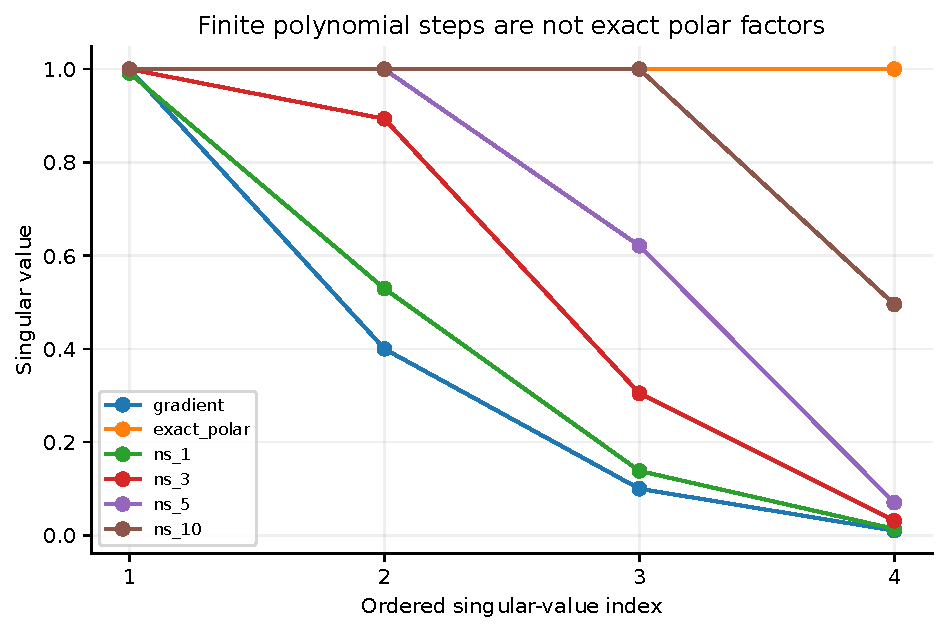
\includegraphics[width=0.85\textwidth]{figures/polar_approximation.pdf}
 \caption{有限步三次 Newton--Schulz 迭代与 SVD 构造的 canonical polar 参考之间的区别。精确 polar 将非零奇异值变为一，并使零奇异方向保持为零；有限步近似在小奇异值方向上可能仍明显偏离参考。因此 NS 步数、初始归一化和数值精度都是所比较算法的一部分。}
 \label{l4:fig-polar-approximation}
\end{figure}

\section{更新 RMS：一种工程尺度，而非迁移定理}
\label{l4:rms-matching}

\subsection{三种缩放约定}

对秩为 $r$ 的 canonical polar 矩阵 $Q\in\R^{m\times n}$，有
\begin{equation}
 \norm{Q}_F^2=r,
 \qquad\operatorname{RMS}(Q)=\sqrt{\frac{r}{mn}}.
 \label{l4:polar-rms}
\end{equation}
若满秩，即 $r=\min(m,n)$，逐元素 RMS 为 $1/\sqrt{\max(m,n)}$。因此以下三个缩放各有不同含义：
\begin{center}
\small
\begin{tabularx}{\textwidth}{lXX}
\toprule
名称 & 式\eqref{l4:muon-reference}中的 $a(m,n)$ & 控制或对齐的尺度\\
\midrule
裸 polar & $1$ & 矩阵更新的谱范数\\
RMS 诱导范数约定 & $\sqrt{m/n}$ & 最坏输入方向的相对 RMS 扰动\\
逐元素 RMS 匹配 & $c\sqrt{\max(m,n)}$ & 满秩精确 polar 的逐元素 RMS 为 $c$\\
\bottomrule
\end{tabularx}
\end{center}
本讲 GPU 实验采用第三种约定，取 $c=0.2$。满秩且使用精确 polar 时，未乘学习率的更新 RMS 恰为 $0.2$；秩亏或有限步 NS 时不必精确等于该值。比较宽度、矩阵形状和学习率时，应同时保留 $a(m,n)$，不能仅抄一个名义学习率。

\subsection{为什么有时观察到 Adam 更新 RMS 接近 $0.2$}

先分析一个用于建立直觉的理想噪声模型。单坐标梯度在时间上独立同分布，均值为零、方差为 $\sigma_g^2>0$；忽略初始瞬态和 $\epsilon$。在稳态，Adam 的两个 EMA 满足
\begin{equation}
 \E m_t^2=\frac{1-\beta_1}{1+\beta_1}\sigma_g^2,
 \qquad \E v_t=\sigma_g^2.
 \label{l4:adam-moment-rms}
\end{equation}
分母和分子由同一历史梯度产生，通常相关，故下面是\emph{近似}而非恒等式：
\begin{equation}
 \E\left[\frac{m_t^2}{v_t}\right]
 \approx\frac{\E m_t^2}{\E v_t}
 =\frac{1-\beta_1}{1+\beta_1}.
 \label{l4:mean-field-rms}
\end{equation}
取 $\beta_1=0.9$，由此预测更新 RMS 约为
$\sqrt{0.1/1.9}\approx0.2294$。它解释了一个可能的量级，并不证明所有数据、模型和训练阶段都具有这个数值。

若第 $j$ 个坐标有非零均值 $\mu_j$ 和噪声方差 $\sigma_j^2$，同样近似给出
\[
 \E u_j^2\approx
 \frac{\mu_j^2+\frac{1-\beta_1}{1+\beta_1}\sigma_j^2}
 {\mu_j^2+\sigma_j^2}.
\]
整体逐元素 RMS 平方应再对这些\emph{比值}作坐标平均，一般不能直接改成两个总和的比值。恒定非零梯度的极限给出更新 RMS 接近一；时间相关的噪声也会改变 $m_t$ 的方差。$\beta_2$ 在式\eqref{l4:mean-field-rms}中消失，是近似结构造成的，不能推断真实分布完全不依赖它。

\citet{Liu2025}在所研究的大模型训练设置中观察到 AdamW 更新 RMS 常在 $0.2$ 到 $0.4$ 附近，并用实验比较支持将 Muon 缩放到相近范围。我们据此把 RMS 匹配作为初始化调参的策略，不把它提升为跨优化器最优超参数必然一致的定理。

\subsection{同样的 RMS 为什么不够，选读}

即使只分析权重的稳态方差，更新的时间相关性也重要。考虑标量递推
\[
 \theta_{t+1}=a\theta_t-\eta u_t,
 \qquad a=1-\eta\lambda,\quad |a|<1.
\]
设 $u_t$ 为零均值平稳过程，$C_k=\Cov(u_t,u_{t-k})$，并假设相关级数使下式收敛。从线性滤波表示
$\theta_t=-\eta\sum_{j\geq0}a^ju_{t-1-j}$ 得到
\begin{equation}
 \Var(\theta_t)=\frac{\eta^2}{1-a^2}
 \left(C_0+2\sum_{k\geq1}a^kC_k\right).
 \label{l4:correlated-update-variance}
\end{equation}
匹配 RMS 只匹配 $C_0$，没有匹配后面的相关项。对真实训练，更新方向与当前梯度、曲率、特征变化的关系也会改变进展。两个更新可以长度相同，一个沿下降方向，另一个几乎正交于梯度；它们不会产生相同训练效果。

因此 RMS 匹配解决的是“把初始搜索放到可比较的尺度附近”，最优学习率和衰减仍应按共同的验证协议选择。观察到某个任务上可复用参数，是有价值的实验结果，但适用范围应与数据和模型设置一起报告。

\section{自然梯度、K-FAC 与 Shampoo：补充阅读}
\label{l4:second-order-optional}

本节不作为课堂必推内容。它提供一个位置明确的研究地图：有的方法用函数分布变化定义度量，有的方法对梯度历史构造结构化预条件。二者都可以节省相对于完整参数空间矩阵的计算，但使用的统计对象不同。

\subsection{自然梯度与 Fisher 度量}

对条件概率模型 $p_w(y\mid x)$，相邻参数之间的模型 KL 散度在适当正则条件下具有局部展开
\[
 \E_x\operatorname{KL}(p_w(\cdot\mid x)\|p_{w+d}(\cdot\mid x))
 =\frac12d^\top\mathcal I(w)d+o(\norm d^2),
\]
其中 Fisher 信息矩阵为
\[
 \mathcal I(w)=\E_x\E_{y\sim p_w(\cdot\mid x)}
 [s_w(x,y)s_w(x,y)^\top],\qquad
 s_w(x,y)=\nabla_w\log p_w(y\mid x).
\]
将式\eqref{l4:quadratic-model}中的度量换成 Fisher，即得到自然梯度的局部思想。矩阵可能奇异，实际应用通常需要阻尼或其他求解处理。Fisher 的数值矩阵会随参数化改变；几何不变性涉及相应变换下的理想方向或连续流，而不是说所有坐标中的矩阵元素都相同。有限步长、阻尼和近似还会改变这种性质\citep{Martens2020}。

还须区分模型分布下的 Fisher 与把训练样本损失梯度做外积得到的经验矩阵。后者常用于计算，但与前者一般不同；不能仅因二者都半正定，就都称为真实 Hessian。

\subsection{K-FAC 的因子化近似}

对一层 $h=Wx$，若输出端反传向量为 $\delta$，单样本矩阵梯度是 $G=\delta x^\top$，因此
\[
 \operatorname{vec}(G)=x\otimes\delta.
\]
对应外积矩阵具有 $xx^\top\otimes\delta\delta^\top$ 的结构。K-FAC 类型方法用
\[
 \E[xx^\top\otimes\delta\delta^\top]
 \approx\E[xx^\top]\otimes\E[\delta\delta^\top]
\]
近似相关块，再通过左右小矩阵求解代替完整大矩阵求逆。若两个因子 $A$ 与 $B$ 均正定，理想无阻尼方向具有 $B^{-1}GA^{-1}$ 的形式；因子奇异时，需要阻尼或明确的广义逆约定。这项期望分离需要检验，不能由单样本梯度是外积自动推出。

\subsection{Shampoo 与当前梯度 polar 的准确关系}

Shampoo 的矩阵版本维护累计统计量\citep{Gupta2018}
\begin{align}
 L_t&=\epsilon I_m+\sum_{s=1}^{t}G_sG_s^\top,\notag\\
 R_t&=\epsilon I_n+\sum_{s=1}^{t}G_s^\top G_s,\notag\\
 D_t&=-\eta_tL_t^{-1/4}G_tR_t^{-1/4}.
 \label{l4:shampoo}
\end{align}
这里 $\epsilon>0$ 使逆幂有定义。其历史统计量不同于只使用当前梯度的矩阵。

如果专门构造一个无阻尼、仅用当前 $G$ 的理想表达式，并把奇异零空间上的负幂解释为零，则有
\begin{equation}
 \bigl((GG^\top)^\dagger\bigr)^{1/4}
 G\bigl((G^\top G)^\dagger\bigr)^{1/4}=Q(G).
 \label{l4:instant-shampoo-polar}
\end{equation}
这里 $A^\dagger$ 表示 Moore--Penrose 伪逆，所以 $(A^\dagger)^{1/4}$ 在正特征值上取 $-1/4$ 次幂、在零特征值上取零。为核对它，把紧致 SVD 代入，左右两边分别贡献 $\Sigma_r^{-1/2}$，于是中间的乘积为
\[
 U_r\Sigma_r^{-1/2}\Sigma_r\Sigma_r^{-1/2}V_r^\top
 =U_rV_r^\top.
\]
这个恒等式清楚连接了瞬时左右预条件与谱球最陡方向，但不能删除“当前梯度、无阻尼、伪逆解释”三个条件后声称完整 Shampoo 等于 Muon。后者还使用动量和有限步近似。

\section{实验：比较更新几何，而不只比较最终损失}
\label{l4:lab}

本实验占一个半学时。先做无需训练的线性代数检查，再在小型神经网络上比较可复现配置。线性代数检查用于发现概念或实现错误；训练实验用于回答在所选数据和预算下哪种配置更有效。

\subsection{实验 A：方向与近似误差}

\begin{enumerate}
 \item 对 $g=(3,-1)^\top$，计算三种范数球方向，核对约束值和一阶损失变化。将坐标作一次正交旋转，检查普通归一化梯度与逐元素 sign 的变换是否相同。
 \item 构造具有指定奇异值的方阵和长方阵，比较 $G$、$Q(G)$、NS1、NS5、NS10 的奇异值、谱范数、Frobenius 范数和逐元素 RMS。加入一个精确秩亏矩阵，确认实现没有把零奇异方向当作需要补齐的正交基。
 \item 对同一个 $G$，分别采用裸 polar、RMS 诱导缩放和 $0.2\sqrt{\max(m,n)}$ 缩放。核对更新谱范数与 RMS，说明哪一种量被保持为常数。
\end{enumerate}

若使用 GPU，先用较高精度的小矩阵结果作为参考，再检查训练采用的精度。这里只要求验证核心数学对象，不要求把课堂版三次 NS 调成最快的竞速实现。

\subsection{实验 B：小型 tanh MLP 的共同协议}

配套训练实验采用小型 tanh MLP，比较 SGD、AdamW 和本讲定义的 Muon。为隔离更新几何，默认权重衰减为零；改变权重衰减属于后续单独消融。所有配置使用相同的数据划分、初始参数、批次顺序与训练步数，每种优化器使用配套配置中预先声明的三组学习率，按统一验证规则选择；测试集只在配置选定后评价。

Muon 只更新前两层的二维权重矩阵；bias 和最终 readout 由 AdamW 更新，辅助学习率必须单独记录。矩阵动量采用
$M_t=\beta M_{t-1}+(1-\beta)G_t$，方向同时提供 SVD 参考和式\eqref{l4:ns-cubic}的有限步实现，默认 NS5，缩放为 $0.2\sqrt{\max(m,n)}$。这些约定定义了本实验的算法，结果不应泛称为所有 Muon 变体的表现。

\begin{center}
\small
\begin{tabularx}{\textwidth}{lXX}
\toprule
比较项目 & 必须固定或记录 & 解释目的\\
\midrule
资源预算 & 批次流、步数、样本数、实际时间 & 分开数据效率与计算效率\\
优化器状态 & 动量、二阶矩参数、$\epsilon$、辅助学习率 & 保证算法名称对应完整公式\\
更新尺度 & 各层 $\operatorname{RMS}(\Delta W)$、$\norm{\Delta W}_{\rm op}$ & 检查名义学习率与实际位移\\
训练结果 & 训练损失、验证损失、选定后的测试结果 & 区分优化与泛化\\
数值近似 & SVD 或 NS 步数、精度、方向误差 & 识别近似质量与成本\\
\bottomrule
\end{tabularx}
\end{center}

理论中的更新 RMS 通常指 $u_t$ 或 $a(m,n)Q_t$，不包含学习率和权重衰减；实际参数位移包含这些因素。实验日志应分别命名，避免用两个不同量验证同一个预测。检查运行时间时，还应排除首次编译和设备初始化的明显影响，并报告测量方式。

\subsection{实验讨论与提交要求}

提交一组方向检查结果、一张统一预算下的训练与验证曲线，以及一张配置表。讨论至少回答以下问题：不同优化器的最优候选学习率是否相同？RMS 匹配后实际特征变化是否相同？NS5 和 SVD 的差别是否集中在小奇异值方向？若两种方法训练损失接近但运行时间不同，应该怎样报告结论？

不要求实验必须出现 Muon 优于 AdamW 的排序。这个小数据、固定架构和有限预算的实验用于核验更新机制及比较协议，不能独自支持大模型上的普遍性能判断。若结果与初始预测不同，优先检查参数组、平均损失约定、尺度因子和有限步近似，再讨论算法机制。

\section{习题}
\label{l4:exercises}

\begin{exercise}[二次度量与范数球]
\label{l4:ex-metric}
推导式\eqref{l4:quadratic-model}的解，并说明为什么 $M$ 不定时问题可能没有有限最小值。对 $\psi(d)=\norm d_\infty$，分别求固定半径球模型和平方范数惩罚模型的一个解，比较其长度因子。
\end{exercise}

\begin{exercise}[Adam 与 sign 的边界]
\label{l4:ex-adam}
在正文两步例子中，保持 $\beta_1=0.9$，把第二个梯度写为 $g_2=-c$，其中 $c>0$。求使第二步 Adam 的更新方向与当前 SignGD 相反的 $c$ 范围。说明该结论为什么与二阶矩的具体正值无关，并列出 Adam 严格化为 SignGD 所需的特例条件。
\end{exercise}

\begin{exercise}[解耦衰减]
\label{l4:ex-decay}
对固定正定预条件矩阵 $P$，证明耦合欧氏 L2 正则与同系数解耦衰减对所有参数 $w$ 等价，当且仅当 $P=I$（假设 $\eta\lambda>0$）。如果允许改变正则化的二次型，找出一个能在固定 $P$ 下产生各向同性衰减的正则项。
\end{exercise}

\begin{exercise}[谱球的解与秩亏]
\label{l4:ex-polar}
对 $G=\diag(4,0)$，给出由 canonical polar 得到的下降方向，以及另一个不同的谱球最优解，取半径一。计算两者的 Frobenius 范数，说明为什么只报告谱球最优值不能唯一确定更新 RMS。再说明 SVD 参考实现应采用什么约定。
\end{exercise}

\begin{exercise}[Newton--Schulz 与 RMS]
\label{l4:ex-ns}
证明对 $0<s<1$ 有 $s<p(s)<1$。若一个 $3\times12$ 的矩阵秩为二，求其 canonical polar 的 RMS，以及乘 $0.2\sqrt{12}$ 后的 RMS；解释为何它不是 $0.2$。讨论 NS5 是否会使该 RMS 必然等于精确 polar 的 RMS。
\end{exercise}

\begin{exercise}[更新长度不足以决定训练动力学]
\label{l4:ex-rms}
给出两个具有相同 RMS 的二维更新向量，使其中一个在指定非零梯度处有严格一阶下降，另一个的一阶变化为零。选读：设标量更新过程的协方差为 $C_k=\sigma_u^2r^{|k|}$，其中 $|r|<1$，把它代入式\eqref{l4:correlated-update-variance}，求权重稳态方差；与白噪声 $r=0$ 比较。
\end{exercise}

\section{习题解答要点}
\label{l4:solutions}

\subsection*{习题\ref{l4:ex-metric}}
一阶条件为 $g+Md/\eta=0$，正定性保证唯一最小值。若 $M$ 有负特征值，沿相应方向二次项趋于负无穷，通常不存在有限最小值。无穷范数球模型的一个解是
$-\rho\operatorname{sign}(g)$；平方范数惩罚模型的一个解是
$-\eta\norm g_1\operatorname{sign}(g)$。两者方向相同，但长度因子分别是固定预算与依赖梯度的 $\eta\norm g_1$。

\subsection*{习题\ref{l4:ex-adam}}
有 $m_2=0.09-0.1c$，偏差修正因子为正，二阶矩分母也为正。因此 $0<c<0.9$ 时 $m_2>0$，Adam 位移为负，而当前 SignGD 位移为正。$c=0.9$ 时一阶矩恰为零。严格的无历史特例为 $\beta_1=\beta_2=0$、$\epsilon=0$，并在零梯度分量上另作约定；恒定梯度且按零初始状态做偏差修正也是一个特殊情形。

\subsection*{习题\ref{l4:ex-decay}}
两种正则贡献分别为 $-\eta\lambda Pw$ 和 $-\eta\lambda w$。要求对所有 $w$ 相同，等价于 $P=I$。若 $P$ 固定，可以使用
$R(w)=\lambda w^\top P^{-1}w/2$，此时 $P\nabla R(w)=\lambda w$。若 $P$ 随参数或历史变化，这个固定二次型解释一般不再成立。

\subsection*{习题\ref{l4:ex-polar}}
canonical polar 为 $D_0=\diag(1,0)$；用于最小化的方向是 $-D_0$。另一个最优解为 $D_1=\diag(-1,1)$：谱范数为一，且 $\inner{G}{D_1}_F=-4$。$\norm{-D_0}_F=1$，$\norm{D_1}_F=\sqrt2$，所以 RMS 不同。SVD 参考实现若要与本讲的 $Q(G)$ 一致，必须将零奇异方向的更新置零，不能任意补成完整正交矩阵。

\subsection*{习题\ref{l4:ex-ns}}
由 $p(s)-s=s(1-s^2)/2>0$ 与
$1-p(s)=(1-s)^2(s+2)/2>0$ 得到所需不等式。
秩二矩阵的 polar RMS 为 $\sqrt{2/36}=1/\sqrt{18}$，缩放后的 RMS 为
$0.2\sqrt{2/3}$。满秩假设不成立，所以不等于 $0.2$。三次 NS 从正奇异值不超过一的初始矩阵出发，有限步非零奇异值通常仍小于一，因此其 RMS 通常还低于相应精确 polar 的值。

\subsection*{习题\ref{l4:ex-rms}}
取梯度 $g=(1,0)^\top$，更新 $d_1=(-1,0)^\top$ 与 $d_2=(0,1)^\top$，两者 RMS 都为 $1/\sqrt2$，而一阶变化分别为 $-1$ 与零。选读部分用几何级数得到
\[
 \Var(\theta)=\frac{\eta^2\sigma_u^2}{1-a^2}
 \frac{1+ar}{1-ar}.
\]
即使 $C_0=\sigma_u^2$ 固定，$r$ 变化仍会改变稳态方差。例如 $0<a,r<1$ 时，该方差大于白噪声情形。这从一个可精确计算的模型说明了 RMS 匹配不等于动力学匹配。

\begin{coursebox}{通向参数化与架构设计}
二次度量说明坐标怎样改变优化路径；对偶范数说明位移预算怎样改变最陡方向；矩阵结构说明参数如何作为线性映射作用于数据。下一讲把这些内容进一步放到函数变化中：架构与参数化改变 Jacobian，优化器改变更新的几何，数据决定哪些函数方向与目标相关。缩放规律必须与这些对象一起定义，才能成为可迁移、可检验的设计原则。
\end{coursebox}
